%%%%%%%%%%%%%%%%%%%%%%%%%%%%%% -*- Mode: Latex -*- %%%%%%%%%%%%%%%%%%%%%%%%%%%%
%% project-description.tex -- 
%% Author          : Robert Brewer
%% Created On      : Wed Jan 27 16:28:11 1999
%% Last Modified By: Robert Brewer
%% Last Modified On: Mon Feb  1 14:16:44 1999
%% RCS: $Id: project-description.tex,v 1.5 1999/02/02 04:02:05 rbrewer Exp $
%%%%%%%%%%%%%%%%%%%%%%%%%%%%%%%%%%%%%%%%%%%%%%%%%%%%%%%%%%%%%%%%%%%%%%%%%%%%%%%
%%   Copyright (C) 1999 Robert Brewer
%%%%%%%%%%%%%%%%%%%%%%%%%%%%%%%%%%%%%%%%%%%%%%%%%%%%%%%%%%%%%%%%%%%%%%%%%%%%%%%
%% 

\setlength{\oddsidemargin}{0in}
\setlength{\textwidth}{7in}

\section{Project Description}
%No more than 1000 words, currently 995 words

\subsection{Introduction}
% 97 words
There is increasing pressure in education to provide high-quality instruction
despite shrinking budgets. Most educators agree that one of best ways to
improve instruction is to increase student-instructor interaction. One of the
most effective technologies for improving interaction between students and
instructors is the electronic mailing list. This approach can improve
instruction in standard courses and is particularly helpful for distance
education where such lists play a crucial role. Generally the instructor will
set up a mailing list for the course, and all the students subscribe to the
list. Students find it easy to participate from home or from labs at school.

\subsection{The Problem With Class Mailing Lists}
%What problem are you solving?
% 89 words
The problem with class mailing lists is that at the end of a semester all the
discussion (and therefore effort) by instructors and students is thrown away.
Even when the messages from the list have been archived, the unorganized pile
of messages is of limited utility to students or instructors for future
semesters. What is needed is a way for this mass of unstructured information to
be turned into an archive which the instructor and future students can learn
from and build on.

\subsection{Condensation \& MCS as a Solution}
%What is the solution to the problem?
% 98 words
I have developed a technique called {\em condensation} whereby a human editor
uses an editing program to: choose which messages to archive, annotate the
archived messages with additional information to make searching the archive
easy, and possibly edit the messages themselves to remove any incorrect or
irrelevant information. I call this complete system (editing tool and
web-accessible archive) MCS: Mailinglist Condensation System. MCS is a part of
my ongoing masters thesis in ICS, more information is available at
\url{<http://csdl.ics.hawaii.edu/Research/MCS/MCS.html>}.

\subsubsection{Example of MCS Use in a Classroom Setting}
%How will it actually work?
% 143 words (including figure caption)
Kimo is taking ICS 111, and is stumped by an error message he received while
trying to compile his homework assignment. It's 11:10 PM, the assignment is due
at midnight, and he needs an answer fast! So he brings up his web browser and
goes to the MCS archive for the class. The archive has been maintained by a
series of instructors who have taught the course over the last 3 years. He
types in the error message into the ``Symptom'' field of the web form, and
clicks the ``Search'' button. The result is a table containing problems with
symptoms similar to Kimo's, and also their solutions as accumulated over time
(see figure \ref{fig:mcs-screenshot}). Kimo learns how to solve his problem and
turn in the assignment just before the deadline.

\begin{figure}[htb]
  \centering
  \includegraphics{mcs-screenshot.eps}
  \caption{Mockup of MCS symptom-based problem lookup}
  \label{fig:mcs-screenshot}
\end{figure}

% 56 words
This example illustrates just one possible data representation taken from one
domain (problem-solution pairs in computer programming). MCS has a number of
additional representations and can support a broad variety of domains. MCS can
be equally useful in non-technical domains such as English composition where
the archive would contain writing examples and common writing problems.

\subsection{Business Plan}
%How will this make money?
%What is the revenue potential?
%What is the potential market?
% 281 words
I intend to release MCS under an {\em Open Source} license. Making a product
open source means that the program is freely redistributable, the source code
is freely available, and other people are free to improve the product. Popular
examples of open source are the Linux operating system and the Apache web
server.

It might seem strange that my business plan starts by giving away the software
for free! However, the open source movement has demonstrated that it {\em is} a
viable way to make money. The money is made by providing service and support to
customers, not in the distribution of the actual software.

Distributing free software via the Internet has substantial marketing
advantages since it allows users to download and evaluate the package without
cost.  However, many instructors will not have the time, expertise, or
institutional support to set up and maintain the archive. One solution is a
``service subscription'', whereby the institution contracts with my company to
provide ongoing support and enhancements. Another potential profit center is
the textbook industry. A special MCS database could be supplied on CD-ROM with
the text (or made available online) as a `seed' archive that would be
`localized' over time through additions by students and instructors. My company
would contract with the textbook publisher to provide the initial database,
with revenues generated from royalties on the text.

Given the number of educational institutions in the US and the growing emphasis
on distance education, I feel there is an enormous market for these support and
editing services. Since these services can be provided remotely via the Internet,
the overhead of such the business would be very low.

\subsection{Competing Technologies}
%Why is your solution unique?
% 80 words
There are effectively no competing systems in this area. Obviously an
instructor could manually assemble a ``Frequently-Asked Questions'' document
for a class, but this still doesn't address the problems of continuous updating 
and efficient searching by students.

There are also web-based instructional support systems like MAILE (Manoa Advanced
Interactive Learning Environment) here at UHM. These systems may provide
improved accessibility to discussion, but they provide no tools for condensing
information over multiple semesters.

%Why Open Source will crush any nascent commercial competition

%Risks in marketing

%Next steps/scale up


\subsection{Project Plan}
%What is the timeline for the project?
%What milestones are there along the way to completion?
%What are the deliverables?
% 91 words

I will be working on this project after the completion of my thesis in Summer
1999. After the completion of my thesis, I will ``clean up'' MCS so that it can
be made available for open source distribution. Working with Professor Johnson
(my advisor), I will set up MCS condensed web sites for class mailing lists
that he has archived. I expect to have the archives ready by the early Fall
1999. He has agreed to pilot the MCS system in his two scheduled classes for
Fall 1999.

\subsubsection{Deliverables}
% 51 words
By the end of the grant award period, I expect to have a version of MCS
suitable for open source distribution, a working server which distributes MCS,
one or more condensed class mailing list archives available on this server, and
a technical report relating the lessons learned in the process.

%Exiled Text:

%There is increasing pressure in academia to provide high-quality education to a
%geographically diverse student population, despite shrinking budgets. There are
%many possible approaches to solving this problem, but one that has gotten a lot
%of focus of late is distance education. Simply put, distance education attempts
%to reach out to students who are not well served by traditional educational
%vicissitudes: professionals who work during the day, and those who are unable
%to travel to the educational institution. In most cases this is done through
%the use of enabling technologies like videoconferencing, real-time chat, and
%electronic mail. I have been involved in two distance learning classes in the
%ICS department (one was ICS 613 in spring 1998, the other is ICS 691 in spring
%99). Both meet once a week for only 90 minutes. Because of the very limited
%face-to-face interaction time, both have an associated electronic mailing list
%which all the students subscribe to. Students use these mailing lists to ask
%questions of the instructor (or each other), and to discuss issues raised
%during class time or by readings. In some cases the instructor will reply with
%answers to the questions, but quite often the answer is sent by another
%student. These mailing lists are a critical part of the courses, and I have
%found their existence to substantially enhance the quality of the educational
%experience.

%For instructors, the problem happens at the end of a course. Throughout the
%semester the instructor and the students have spent countless hours answering
%questions and synthesizing new insights into the material. But at the end of
%the semester, all that remains is file containing all the messages sent to the
%mailing list (if someone had the foresight to start the archival at the
%beginning of the course). In this format the messages are of very little
%utility to future students, or the instructor. Even if the instructor were to
%take the time to sift through all the messages and delete the redundant or
%irrelevant ones, there is still no way for a future student to determine
%whether his or her question is answered in the archive.
% LocalWords:  http Kimo tex Mailinglist csdl ics hawaii edu html Kimo's htbp
% LocalWords:  mcs eps redistributable CD MAILE LocalWords videoconferencing
% LocalWords:  htb
